%% This is file `elsarticle-template-1-num.tex',
%%
%% Copyright 2009 Elsevier Ltd
%%
%% This file is part of the 'Elsarticle Bundle'.
%% ---------------------------------------------
%%
%% It may be distributed under the conditions of the LaTeX Project Public
%% License, either version 1.2 of this license or (at your option) any
%% later version.  The latest version of this license is in
%%    http://www.latex-project.org/lppl.txt
%% and version 1.2 or later is part of all distributions of LaTeX
%% version 1999/12/01 or later.
%%
%% The list of all files belonging to the 'Elsarticle Bundle' is
%% given in the file `manifest.txt'.
%%
%% Template article for Elsevier's document class `elsarticle'
%% with numbered style bibliographic references
%%
%% $Id: elsarticle-template-1-num.tex 149 2009-10-08 05:01:15Z rishi $
%% $URL: http://lenova.river-valley.com/svn/elsbst/trunk/elsarticle-template-1-num.tex $
%%
\documentclass[final,10pt]{elsarticle}


%% Use the option review to obtain double line spacing
%% \documentclass[preprint,review,12pt]{elsarticle}

%% Use the options 1p,twocolumn; 3p; 3p,twocolumn; 5p; or 5p,twocolumn
%% for a journal layout:
%% \documentclass[final,1p,times]{elsarticle}
%% \documentclass[final,1p,times,twocolumn]{elsarticle}
%% \documentclass[final,3p,times]{elsarticle}
%% \documentclass[final,3p,times,twocolumn]{elsarticle}
%% \documentclass[final,5p,times]{elsarticle}
%% \documentclass[final,5p,times,twocolumn]{elsarticle}

%% if you use PostScript figures in your article
%% use the graphics package for simple commands
%% \usepackage{graphics}
%% or use the graphicx package for more complicated commands
%% \usepackage{graphicx}
%% or use the epsfig package if you prefer to use the old commands
%% \usepackage{epsfig}

%% The amssymb package provides various useful mathematical symbols
\usepackage{amssymb}
%% The amsthm package provides extended theorem environments
%% \usepackage{amsthm}

\usepackage{booktabs}
%\usepackage{amsmath}
\usepackage{mathtools}
\usepackage{amssymb}
\usepackage{longtable}

%% The lineno packages adds line numbers. Start line numbering with
%% \begin{linenumbers}, end it with \end{linenumbers}. Or switch it on
%% for the whole article with \linenumbers after \end{frontmatter}.
\usepackage{lineno}

%% natbib.sty is loaded by default. However, natbib options can be
%% provided with \biboptions{...} command. Following options are
%% valid:

%%   round  -  round parentheses are used (default)
%%   square -  square brackets are used   [option]
%%   curly  -  curly braces are used      {option}
%%   angle  -  angle brackets are used    <option>
%%   semicolon  -  multiple citations separated by semi-colon
%%   colon  - same as semicolon, an earlier confusion
%%   comma  -  separated by comma
%%   numbers-  selects numerical citations
%%   super  -  numerical citations as superscripts
%%   sort   -  sorts multiple citations according to order in ref. list
%%   sort&compress   -  like sort, but also compresses numerical citations
%%   compress - compresses without sorting
%%
%% \biboptions{comma,round}

% \biboptions{}


\journal{Journal Name}

\begin{document}
\pagenumbering{gobble}

\begin{frontmatter}

%% Title, authors and addresses

%% use the tnoteref command within \title for footnotes;
%% use the tnotetext command for the associated footnote;
%% use the fnref command within \author or \address for footnotes;
%% use the fntext command for the associated footnote;
%% use the corref command within \author for corresponding author footnotes;
%% use the cortext command for the associated footnote;
%% use the ead command for the email address,
%% and the form \ead[url] for the home page:
%%
%% \title{Title\tnoteref{label1}}
%% \tnotetext[label1]{}
%% \author{Name\corref{cor1}\fnref{label2}}
%% \ead{email address}
%% \ead[url]{home page}
%% \fntext[label2]{}
%% \cortext[cor1]{}
%% \address{Address\fnref{label3}}
%% \fntext[label3]{}

\title{Effect of hyperdynamic LVEF on ICU outcomes}

%% use optional labels to link authors explicitly to addresses:
%% \author[label1,label2]{<author name>}
%% \address[label1]{<address>}
%% \address[label2]{<address>}

\author{Joseph Panessa, Thomas Brennan, Marco Pimentel, Mengling Feng, Leo Celi}

\address{Cambridge MA, United States}


\begin{abstract}
%% Text of abstract
\textbf{Objective}
 To study the effect of hyperdynamic left ventricular function on ICU outcomes.

\end{abstract}

\begin{keyword}
Intensive Care Unit \sep Hyperdynamic
%% keywords here, in the form: keyword \sep keyword

%% MSC codes here, in the form: \MSC code \sep code
%% or \MSC[2008] code \sep code (2000 is the default)

\end{keyword}

\end{frontmatter}

%%
%% Start line numbering here if you want
%%
\linenumbers

%% main text
\section{Background}
\label{S:1}
In a recent meta-analysis review by Huang et al.~(2013)~\cite{huang2013early} the 
authors attemped to answer the question whether ventricular depression or dilation is 
associated with lower mortality rates. A total of 62 studies were reviewed and 14 
included in the analysis. The meta-analysis failed to find any evidence to support the 
view that the survivors from severe sepsis or septic shock had lower ejection fractions.
This study aims to further explore this research question using the MIMIC-II clinical 
database from the Beth Israel Deaconness Medical Center in Boston, MA~\cite{SaeedCCM11}.
 

\section{Methods}

We conducted a retrospective cohort study using the Multiparameter 
Intelligent Monitoring in Intensive Care II (MIMIC II) database. 
MIMIC II is a large open-access database, which includes 
data from electronic medical records of patients 
admitted to the ICUs at Beth Israel Deaconess Medical Center since 2001. 
The creation and use of the MIMIC database was approved by the institutional 
review boards of both Beth Israel Deaconess Medical Center and 
Massachusetts Institute of Technology (IRB protocol 2001-P-001699/3).

All adult patient records who underwent an echocardiograph 
in the database were screened for purposes of inclusion. 
Patients were excluded if their left-ventricular function was suppresed 
The cohort characteristics used in this study is shown in Figure~\ref{fig:cohort}. 
The study outcome was 28-day mortality among the entire
patient cohort.

All statistical analysis was performed using R. 
Baseline comparisons were performed using Fisher tests for categorical variables with 
results reported as numbers and percentages. 
Continuously normally distributed variables were compared using \emph{t}-tests and 
reported as median, while non-normally distributed data 
were compared using Mann-Whitney tests and reported as medians and 
interquartile range (IQR).

\begin{figure}[h]
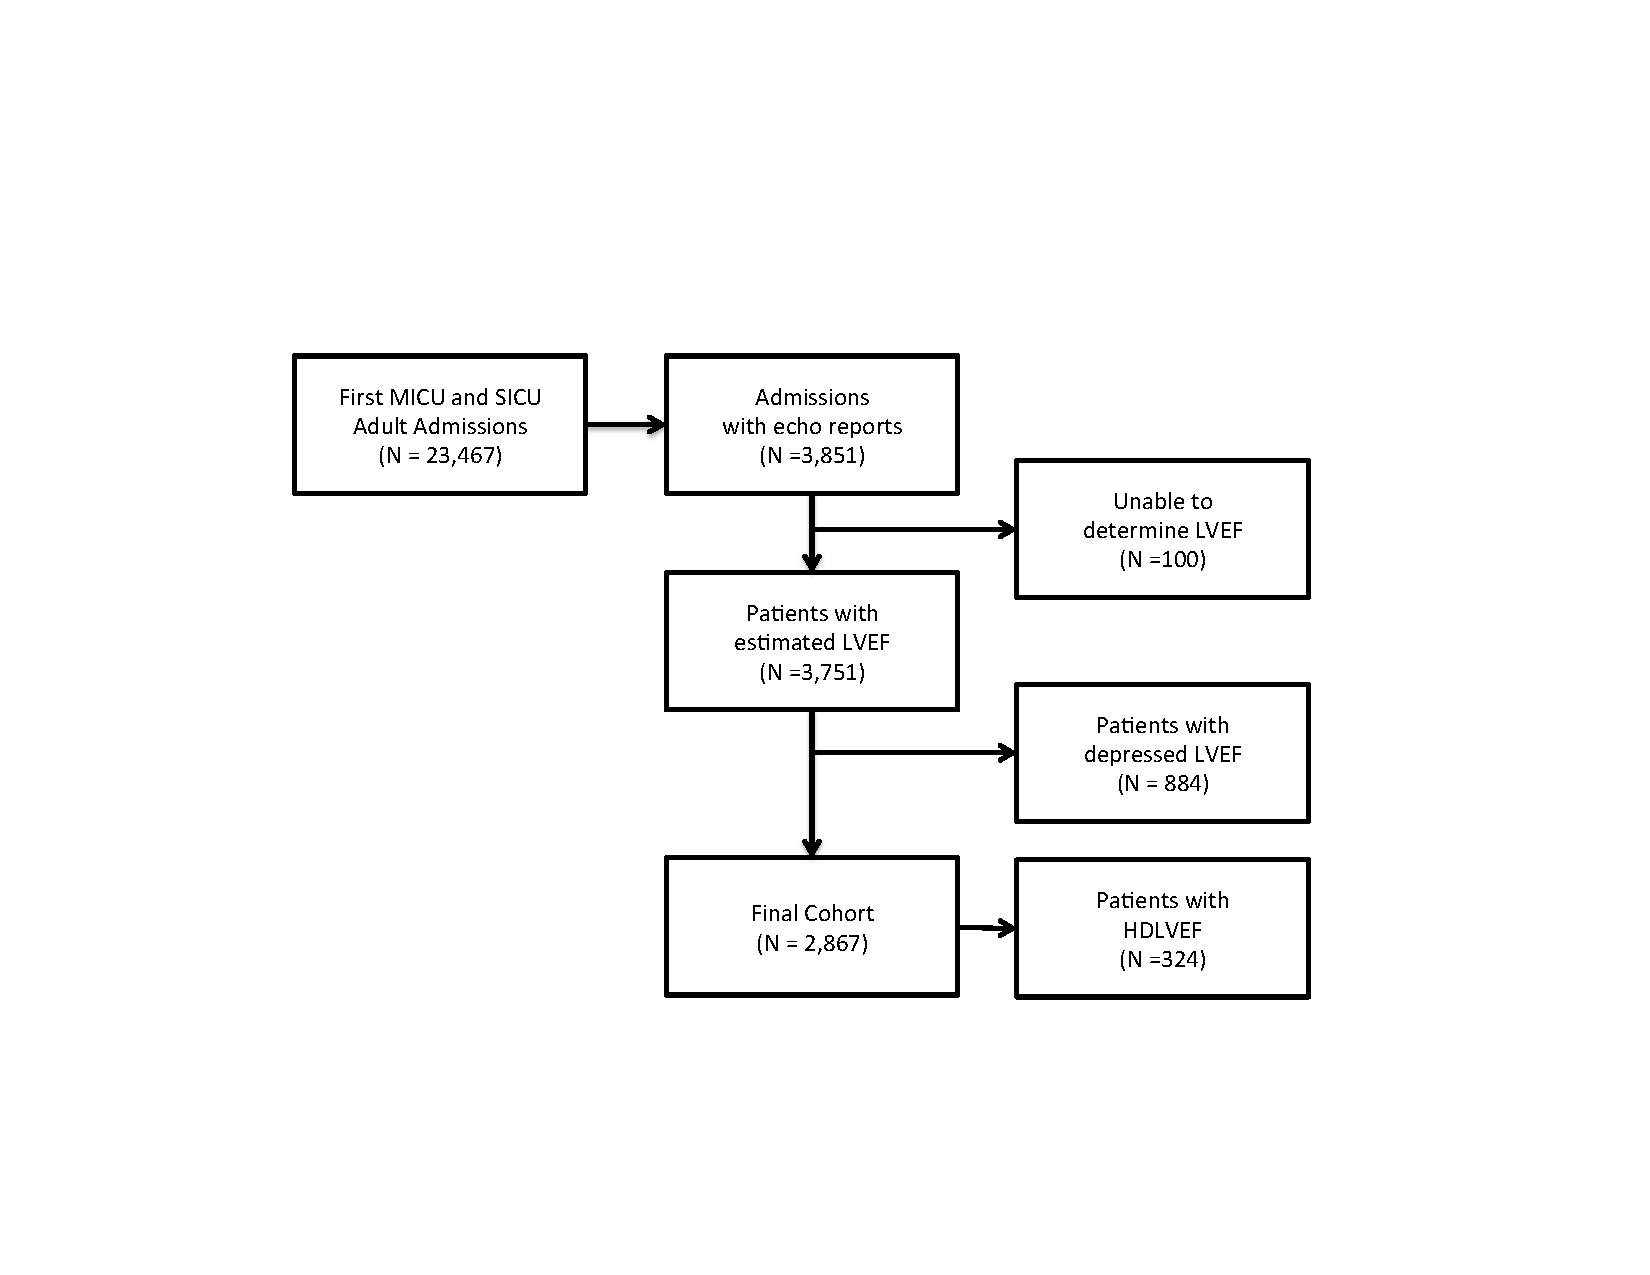
\includegraphics[width=\linewidth,natheight=612,natwidth=792]{../figure/fig_cohort.pdf}
\caption{Patient record selection. Using the MIMIC II database 
we identified 2,481 patients that had a echo report.}
\label{fig:cohort}
\end{figure}

\section{Results}
Table~\ref{tbl1:hypers} highlights the results of the univariate analysis 
for all patients with hyperdynamic EF. Table~\ref{tbl1:acute_hypers} highlights the results of the univariate analysis 
for all patients with acute hyperdynamic EF. Significant values ($P<0.05$) are shown in bold. 
Hyperdynamic patients are more likely to be female, be admitted to MICU, SICU 
and ventilated.
Hyperdynamic patients also have higher risk of mortality, SOFA and SAPSI scores and 
stay longer in ICU. Table~\ref{tbl:all_icd9} looks at potential confounders 
for the cohort: hyperdynamic patients are more liekly to have congestive heart failure, 
hypertension and cancer. 

Table~\ref{tbl:sepsis} highlights the results of the univariate 
analysis for all septic patients. Significant values ($P<0.05$) are shown in bold. 
Hyperdynamic septic patients have a higher 28-day and ICU/hospital mortality are more 
likely to be administered more fluids. The confounder analysis in 
Table~\ref{tbl:sepsis_icd9} is inconclusive.


\begin{table}[h]
\begin{tabular}{l c c c}
\toprule
 & \textbf{NLVEF} (N=3527) & \textbf{HDLVEF} (N=324) & $P$-value\\
 & \multicolumn{2}{c}{N (\%) or median [IQR]} & \\ \hline
Age & 67 [53 - 79] & 69 [56 - 78]&0.6\\
Gender (Male)&1833 (52 \%) & 134 (41 \%)&\textbf{$<$ 0.01}\\
Care Unit& ~ & ~ & 0.9\\
~~MICU&2416 (69 \%)&221 (68 \%)&\\
~~SICU&1111 (31 \%)&103 (32 \%)&\\
Time to echo (days) & 1.1 [0.1 - 3.2] & 0.9 [0.0 - 4.2]&0.5\\
Time to vasopressors (days) & 0.1 [0.0 - 0.4] & 0.1 [0.0 - 0.7]&0.5\\
\multicolumn{3}{l}{Co-morbidities by ICD9 \& DRG Codes}\\
~~Diabetes&860 (24 \%)&89 (27 \%)&0.2\\
~~Alcohol abuse&193 (5 \%)&19 (6 \%)&0.7\\
~~Arrhythmias&1039 (29 \%)&82 (25 \%)&0.1\\
~~Valvular disease&418 (12 \%)&38 (12 \%)&1.0\\
~~Hypertension&1126 (32 \%)&134 (41 \%)&\textbf{$<$ 0.01}\\
~~Renal failure&342 (10 \%)&29 (9 \%)&0.8\\
~~Chronic pulmonary&754 (21 \%)&68 (21 \%)&0.9\\
~~Liver disease&255 (7 \%)&32 (10 \%)&0.1\\
~~Cancer&170 (5 \%)&28 (9 \%)&\textbf{$<$ 0.01}\\
~~Psychosis&142 (4 \%)&15 (5 \%)&0.6\\
~~Depression&177 (5 \%)&12 (4 \%)&0.3\\
~~CHF&1363 (39 \%)&127 (39 \%)&0.9\\
Illness & ~ & ~ &\\
~~SOFA & 6 [3 - 9] & 7 [4 - 10]&\textbf{$<$ 0.01}\\
~~Septic&1496 (42 \%) & 150 (46 \%)&0.2\\
Vital Signs & ~ & ~ &\\
~~Max HR (bpm)&113 [98 - 130]&120 [102 - 139]&\textbf{$<$ 0.01}\\
~~Median HR Day1 (bpm)&87 [75 - 99]&90 [79 - 105]&\textbf{$<$ 0.01}\\
~~Min MAP&56 [48 - 64]&52 [44 - 62]&\textbf{$<$ 0.01}\\
~~Max Temperature (C)&37.8 [37.3 - 38.5]&37.9 [37.3 - 38.4]&0.4\\
Lab Results & ~ & ~ &\\
~~Max WBC&13.3 [9.6 - 18.4]&14.6 [10.2 - 20.5]&0.01\\
~~Max lactate&2.2 [1.5 - 3.8]&2.6 [1.6 - 4.8]&\textbf{$<$ 0.01}\\
~~Max creatinine&1.1 [0.8 - 2.0]&1.2 [0.8 - 2.0]&0.5\\
Treatments & ~ & ~ &\\
~~Vasopressor&1121 (32 \%)&131 (40 \%)&\textbf{$<$ 0.01}\\
~~Received Dobutamine&92 (9 \%)&13 (11 \%)&0.5\\
~~RRT&414 (12 \%)&50 (16 \%)&0.05\\
~~Ventilated&1767 (51 \%)&195 (62 \%)&\textbf{$<$ 0.01}\\
~~IVF first 24hr (ml) & 2240 [682 - 5142] & 2500 [771 - 5702]&0.2\\
~~IVF first 72hr (ml) & 7339 [3620 - 12582] & 8949 [5108 - 14585]&\textbf{$<$ 0.01}\\

\bottomrule
\end{tabular}
\caption{Characteristics of normal versus all HDLVEF patients}
\label{tbl:hypers}
\end{table}

%\begin{table}[h]
%\begin{tabular}{l c c c}
%\toprule
% & \textbf{NLVEF} (N=2534) & \textbf{HDLVEF} (N=324) & $P$-value\\
 & \multicolumn{2}{c}{N (\%) or median (IQR)} & \\ \hline
Age&64.61 (27.22)&68.59 (22.84)&\textbf{0.03}\\
Gender (Male)&1238 (49.03)&134 (41.49)&\textbf{0.01}\\
SAPS-I&14.00 (7.00)&16.00 (7.00)&\textbf{$<$ 0.01}\\
Care Unit& ~ & ~ & 0.9\\
~~MICU&1713 (67.60)&221 (68.21)&\\
~~SICU&821 (32.40)&103 (31.79)&\\
Time to echo (days)&1.09 (3.22)&0.92 (4.20)&0.4\\
Outcomes & ~ & ~ &\\
~~ICU LOS (days)&3.66 (7.03)&4.33 (11.86)&\textbf{$<$ 0.01}\\
~~HOSP LOS (days)&11.00 (14.00)&16.00 (19.00)&\textbf{$<$ 0.01}\\
\toprule & \textbf{NLVEF} (N=2534) & \textbf{HDLVEF} (N=324) & $P$-value\\
 & \multicolumn{2}{c}{N (\%) or median (IQR)} & \\ \hline
Co-morbidities & ~ & ~ &\\
~~Diabetes&590 (23.28)&89 (27.47)&0.1\\
~~Alcohol abuse&153 (6.04)&19 (5.86)&1.0\\
~~Arrhythmias&700 (27.62)&82 (25.31)&0.4\\
~~Valvular disease&255 (10.06)&38 (11.73)&0.4\\
~~Hypertension&850 (33.54)&134 (41.36)&\textbf{$<$ 0.01}\\
~~Renal failure&213 (8.41)&29 (8.95)&0.8\\
~~Chronic pulmonary&536 (21.15)&68 (20.99)&1.0\\
~~Liver disease&198 (7.81)&32 (9.88)&0.2\\
~~Cancer&119 (4.70)&28 (8.64)&\textbf{$<$ 0.01}\\
~~Psychosis&115 (4.54)&15 (4.63)&0.9\\
~~Depression&148 (5.84)&12 (3.70)&0.1\\
~~CHF&840 (33.15)&127 (39.20)&\textbf{0.03}\\
\toprule & \textbf{NLVEF} (N=2534) & \textbf{HDLVEF} (N=324) & $P$-value\\
 & \multicolumn{2}{c}{N (\%) or median (IQR)} & \\ \hline
Labs & ~ & ~ &\\
~~Max WBC&13.30 (8.90)&14.60 (10.28)&\textbf{$<$ 0.01}\\
~~wbc&11.00 (6.80)&11.53 (7.70)&\textbf{0.02}\\
~~Max lactate&2.10 (2.30)&2.60 (3.15)&\textbf{$<$ 0.01}\\
~~Lactate&1.70 (1.30)&1.90 (1.40)&\textbf{$<$ 0.01}\\
~~Max creatinine&1.10 (1.00)&1.20 (1.20)&\textbf{0.04}\\
~~Creatinine&0.90 (0.80)&1.00 (0.94)&0.1\\
Treatments & ~ & ~ &\\
~~RRT&288 (11.37)&50 (15.43)&\textbf{0.04}\\
~~Vasopressor&850 (33.54)&143 (44.14)&\textbf{$<$ 0.01}\\
~~Ventilated&1339 (52.84)&202 (62.35)&\textbf{$<$ 0.01}\\
~~IVF first 24hr (ml)&2206.63 (4566.65)&2500.00 (4930.78)&0.2\\

%\bottomrule
%\end{tabular}
%\caption{Characteristics of normal versus all HDLVEF patients}
%\label{tbl:hypers}
%\end{table}

%\begin{table}[h]
%\begin{tabular}{l c c c}
%\toprule
% & \textbf{NLVEF} (N=2534) & \textbf{HDLVEF} (N=324) & $P$-value\\
 & N (\%) & N (\%) &\\ \hline
~~Dobutamine&17 (1.93)&4 (3.31)&0.3\\
~~Dopamine&77 (8.75)&11 (9.09)&0.9\\
~~Vasopressin&24 (2.73)&7 (5.79)&0.1\\
~~Levophed&160 (18.18)&29 (23.97)&0.1\\
~~Milrinone&1 (0.11)&0 (0.00)&1.0\\
~~Neosynephrine&114 (12.95)&22 (18.18)&0.1\\

%\bottomrule
%\end{tabular}
%\caption{Characteristics of normal versus all HDLVEF patients}
%\label{tbl:hypers}
%\end{table}

\begin{table}[h]
\begin{tabular}{l c c}
\toprule
~ & Odds-ratio (95\% Confidence Interval) & $P$-value\\ \hline
Age&1.005 (1.000,1.010)&0.1\\
Gender (Male)&1.078 (0.878,1.323)&0.5\\
Elixhauser Score&1.059 (1.042,1.077)&\textbf{$<$0.001}\\
SAPS-I&1.104 (1.082,1.127)&\textbf{$<$0.001}\\
Adjusted Vasopressor Dose&1.972 (1.309,2.982)&\textbf{0.001}\\
HDLVEF&1.415 (1.055,1.882)&\textbf{0.02}\\

\bottomrule
\end{tabular}
\caption{Multivariate logistic regression model predicting 28-day mortality for all patients}
\label{tbl:all-comorb}
\end{table}

\begin{table}[t]
\begin{tabular}{l c c c}
\toprule
~ & Odds-ratio (95\% Confidence Interval) & \textbf{P-value}\\ \hline
Age&1.005 (0.997,1.013)&0.2\\
Gender (Male)&1.202 (0.899,1.610)&0.2\\
Elixhauser Score&1.053 (1.029,1.078)&\textbf{$<$0.001}\\
SAPS-I&1.066 (1.035,1.098)&\textbf{$<$0.001}\\
Vasopressor&1.861 (1.367,2.542)&\textbf{$<$0.001}\\
HDLVEF&1.537 (1.028,2.273)&\textbf{0.03}\\

\bottomrule
\end{tabular}
\caption{Multivariate logistic regression model predicting 28-day mortality for septic patients}
\label{tbl:acute-charac}
\end{table}

\begin{table}[h]
\begin{tabular}{l c c}
\toprule
~ & Hazard ratio (95\% Confidence Interval) & \textbf{P-value}\\ \hline
Age&1.0058 (1.0034,1.0082)&\textbf{$<$0.001}\\
Gender (Male)&1.0661 (0.9796,1.1601)&0.1\\
Elixhauser Score&1.0193 (1.0105,1.0281)&\textbf{$<$0.001}\\
SAPS-I&0.9894 (0.7631,1.2826)&0.9\\
Adjusted Vasopressor Dose&1.0694 (0.9296,1.2302)&0.3\\
HDLVEF&1.0365 (1.0277,1.0454)&\textbf{$<$0.001}\\

\bottomrule
\end{tabular}
\caption{Multivariate Cox Hazard model predicting one-year mortality for all 28-day survivors}
\label{tbl:all-comorb}
\end{table}

% vasopressors _k are the same  
\begin{table}
\begin{tabular}{l c c c}
\toprule
 & \textbf{NLVEF} (N=2534) & \textbf{HDLVEF} (N=324) & $P$-value\\
 & N (\%) & N (\%) &\\ \hline
~~Dobutamine&17 (1.93)&4 (3.31)&0.3\\
~~Dopamine&77 (8.75)&11 (9.09)&0.9\\
~~Vasopressin&24 (2.73)&7 (5.79)&0.1\\
~~Levophed&160 (18.18)&29 (23.97)&0.1\\
~~Milrinone&1 (0.11)&0 (0.00)&1.0\\
~~Neosynephrine&114 (12.95)&22 (18.18)&0.1\\

\bottomrule
\end{tabular}
\caption{Vasopressor use between normal versus all hyperdynamic EF patients}
\label{tbl1:hypers}
\end{table}


%% The Appendices part is started with the command \appendix;
%% appendix sections are then done as normal sections
%% \appendix

%% \section{}
%% \label{}

%% References
%%
%% Following citation commands can be used in the body text:
%% Usage of \cite is as follows:
%%   \cite{key}          ==>>  [#]
%%   \cite[chap. 2]{key} ==>>  [#, chap. 2]
%%   \citet{key}         ==>>  Author [#]

%% References with bibTeX database:

\bibliographystyle{model1-num-names}
\bibliography{../../lcp.bib}

%% Authors are advised to submit their bibtex database files. They are
%% requested to list a bibtex style file in the manuscript if they do
%% not want to use model1-num-names.bst.

%% References without bibTeX database:

% \begin{thebibliography}{00}

%% \bibitem must have the following form:
%%   \bibitem{key}...
%%

% \bibitem{}

% \end{thebibliography}


\end{document}

%%
%% End of file `elsarticle-template-1-num.tex'.
